%%%%%%%%%%%%%%%%%%%%%%%%%%%%%%%%%%%%%%%%%
% Beamer Presentation
% LaTeX Template
% Version 1.0 (10/11/12)
%
% This template has been downloaded from:
% http://www.LaTeXTemplates.com
%
% License:
% CC BY-NC-SA 3.0 (http://creativecommons.org/licenses/by-nc-sa/3.0/)
%
%%%%%%%%%%%%%%%%%%%%%%%%%%%%%%%%%%%%%%%%%

%----------------------------------------------------------------------------------------
%	PACKAGES AND THEMES
%----------------------------------------------------------------------------------------

\documentclass{beamer}


\mode<presentation> {

% The Beamer class comes with a number of default slide themes
% which change the colors and layouts of slides. Below this is a list
% of all the themes, uncomment each in turn to see what they look like.

%\usetheme{default}
%\usetheme{AnnArbor}
%\usetheme{Antibes}
%\usetheme{Bergen}
%\usetheme{Berkeley}
%\usetheme{Berlin}
%\usetheme{boxes}
\usetheme{Boadilla}
%\usetheme{CambridgeUS}
%\usetheme{Copenhagen}
%\usetheme{Darmstadt}
%\usetheme{Dresden}
%\usetheme{Frankfurt}
%\usetheme{Goettingen}
%\usetheme{Hannover}
%\usetheme{Ilmenau}
%\usetheme{JuanLesPins}
%\usetheme{Luebeck}
%\usetheme{Madrid}
%\usetheme{Malmoe}
%\usetheme{Marburg}
%\usetheme{Montpellier}
%\usetheme{PaloAlto}
%\usetheme{Pittsburgh}
%\usetheme{Rochester}
%\usetheme{Singapore}
%\usetheme{Szeged}
%\usetheme{Warsaw}

% As well as themes, the Beamer class has a number of color themes
% for any slide theme. Uncomment each of these in turn to see how it
% changes the colors of your current slide theme.

%\usecolortheme{albatross}
%\usecolortheme{beaver}
%\usecolortheme{beetle}
%\usecolortheme{crane}
%\usecolortheme{dolphin}
%\usecolortheme{dove}
%\usecolortheme{fly}
%\usecolortheme{lily}
%\usecolortheme{orchid}
%\usecolortheme{rose}
%\usecolortheme{seagull}
%\usecolortheme{seahorse}
%\usecolortheme{whale}
%\usecolortheme{wolverine}

%\setbeamertemplate{footline} % To remove the footer line in all slides uncomment this line
%\setbeamertemplate{footline}[page number] % To replace the footer line in all slides with a simple slide count uncomment this line
\definecolor{calpolypomonagreen}{rgb}{0.12, 0.3, 0.17}
\usecolortheme[named=calpolypomonagreen]{structure}
% \setcitestyle{square}
\setbeamertemplate{navigation symbols}{}} % To remove the navigation symbols from the bottom of all slides uncomment this line

\usepackage{amssymb}% http://ctan.org/pkg/amssymb
\usepackage{pifont}% http://ctan.org/pkg/pifont
\newcommand{\cmark}{\textcolor{green}{\ding{51}}}%
\newcommand{\xmark}{\textcolor{red}{\ding{55}}}%

\usepackage{graphicx} % Allows including images
\usepackage{lmodern}
\usepackage{xcolor}
\usepackage{chronology}
\usepackage{appendixnumberbeamer}
\usepackage{pgf}
%\usepackage{smartdiagram}
\usepackage{tikz}
\usepackage{subfigure}
\usepackage{verbatim}
\usepackage{listings}
\usepackage{comment}
\usepackage{pgfgantt}
\usepackage{amsmath}
\usepackage[sort, numbers]{natbib}
\usepackage{moresize}
\usepackage{tikz}
\usetikzlibrary{backgrounds}
\usepackage[absolute,overlay]{textpos}
\usepackage{amssymb}
\usepackage{array}
\usepackage{url}
\usepackage{anyfontsize}
\usepackage{tikz}
\usetikzlibrary{calc}

% tikzmark command, for shading over items
\newcommand{\tikzmark}[1]{\tikz[overlay,remember picture] \node (#1) {};}

\newenvironment{variableblock}[3]{%
  \setbeamercolor{block body}{#2}
  \setbeamercolor{block title}{#3}
  \begin{block}{#1}}{\end{block}}

\newcommand*{\MyBall}{\tikz \draw [baseline, ball color=red, draw=red] circle (2pt);}

\newcommand{\backupbegin}{
   \newcounter{finalframe}
   \setcounter{finalframe}{\value{framenumber}}
}
\newcommand{\backupend}{
   \setcounter{framenumber}{\value{finalframe}}
}
%\AtBeginSection[]{\frametitle{Table of Contents}
%    \tableofcontents[currentsection]}
%\AtBeginSubsection[]{\begin{frame}
%    \frametitle{Table of Contents}
%    \tableofcontents[currentsection,currentsubsection]
%  \end{frame}}

\makeatletter
\newcommand{\rmnum}[1]{\romannumeral #1}
\newcommand{\Rmnum}[1]{\expandafter\@slowromancap\romannumeral #1@}
\makeatother
\newcommand{\highlight}[1]{%
  \colorbox{red!50}{$\displaystyle#1$}}
\newlength{\overwritelength}
\newlength{\minimumoverwritelength}
\setlength{\minimumoverwritelength}{1cm}
\newcommand{\overwrite}[3][red]{%
  \settowidth{\overwritelength}{$#2$}%
  \ifdim\overwritelength<\minimumoverwritelength%
    \setlength{\overwritelength}{\minimumoverwritelength}\fi%
  \stackrel
    {%
      \begin{minipage}{\overwritelength}%
        \color{#1}\centering\small #3\\%
        \rule{1pt}{9pt}%
      \end{minipage}}
    {\colorbox{#1!50}{\color{black}$\displaystyle#2$}}}

%----------------------------------------------------------------------------------------
%	TITLE PAGE
%----------------------------------------------------------------------------------------

\title[WAGASCI/ND280 CC0\pi^{+/-} Analysis]{Status report: Selection Development for joint measurement of CC0$\pi^{+/-}$ ${\nu}_{\mu}$ xsec on C$_8$H$_8$/H$_2$0 with WAGASCI \& ND280} % The short title appears at the bottom of every slide, the full title is only on the title page
%
\author{John Nugent} % Your name
\institute[TU] % Your institution as it will appear on the bottom of every slide, may be shorthand to save space
{Tohoku University\\ % Your institution for the title page
\medskip
\textit{john.nugent.d5@tohoku.ac.jp}} % Your email address
\date{1/11/2023} % Date, can be changed to a custom date
\begin{document}
%
\begin{frame}
\titlepage % Print the title page as the first slide
\end{frame}

%\begin{frame}
%\frametitle{Table of Contents} % Table of contents slide, comment this block out to remove it
%\tableofcontents % Throughout your presentation, if you choose to use %\section{} and \subsection{} commands, these will automatically be printed on this slide as an overview of your presentation
%\end{frame}

%----------------------------------------------------------------------------------------
%	PRESENTATION SLIDES
%----------------------------------------------------------------------------------------

% \begin{frame}{Analysis Motivation}

% \begin{itemize}
%     \item Built WAGASCI at 1.5$^\circ$ off-axis to exploit correlations in flux between different off-axis positions, joint analysis never done with WAGASCI
%     \item Separate flux and xsec effects, study $\bar{\nu}$ xsec as a function of energy
%     \item Want to harness this capability: joint xsec analysis with ND280 \& WAGASCI
%     \item Knowledge of interaction asymmetry between $\nu$ and $\bar{\nu}$ of fundamental importance for CP violation experiment 
%     \begin{itemize}
%         \item Aim to measure oscillation asymmetry between the two. A mismodeling of the interaction differences could introduce biases
%     \end{itemize}
%     \item No clear winner in $\nu$ xsec modeling to date, inconsistencies cannot be fully explained by FSI alone
%     \item Interactions involving correlated nucleons contribute to the observed difference via vector-axial interference, positive for $\nu$ and negative for $\bar{\nu}$
%     \item Measure and understand this term for $\bar{\nu}$ can reduce bias in measurement
% \end{itemize}
% \vfill
% 
% \end{frame}

\begin{frame}{Analysis Motivation}

\begin{itemize}
    \item Built WAGASCI at 1.5$^\circ$ off-axis to exploit correlations in flux between different off-axis positions, joint analysis never done with WAGASCI
    \item Separate flux and xsec effects, study ${\nu}$ xsec as a function of energy
    \item Want to harness this capability: joint xsec analysis with ND280 \& WAGASCI
\end{itemize}

\center 
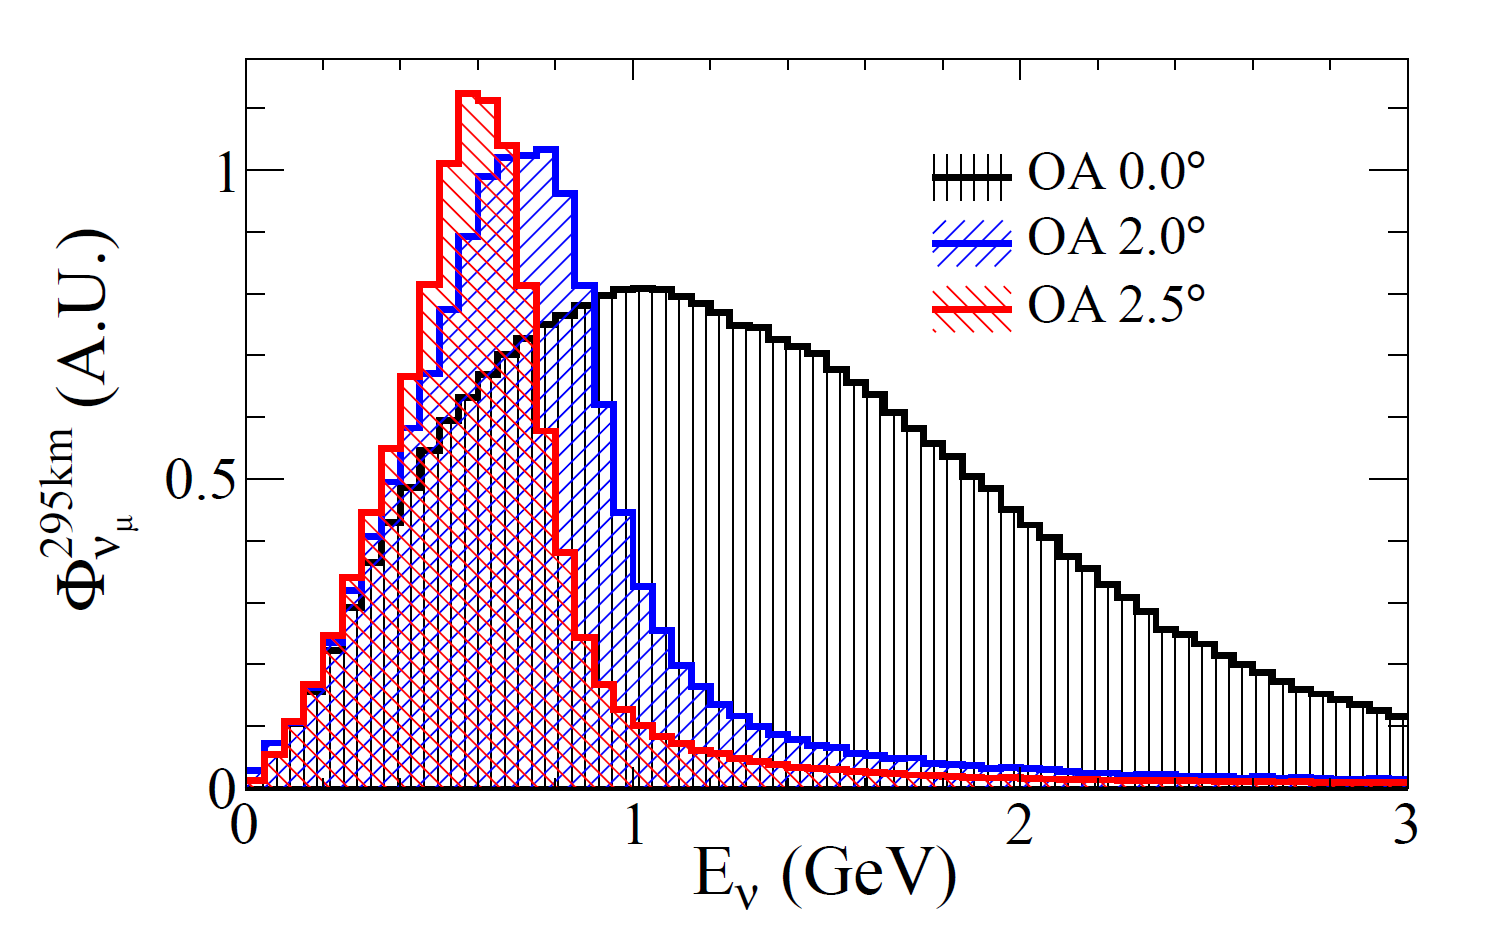
\includegraphics[width=.7\textwidth]{images/figure-t2k-beam-off-axis.png}
\end{frame}

\begin{frame}{WAGASCI}

\begin{itemize}
\item WAGASCI: WAter Grid And SCIntillator detector 
\item Water and scintillator target for carbon and oxygen neutrino cross-sections
\end{itemize}

\begin{columns}[c]
\begin{column}{.5\textwidth}
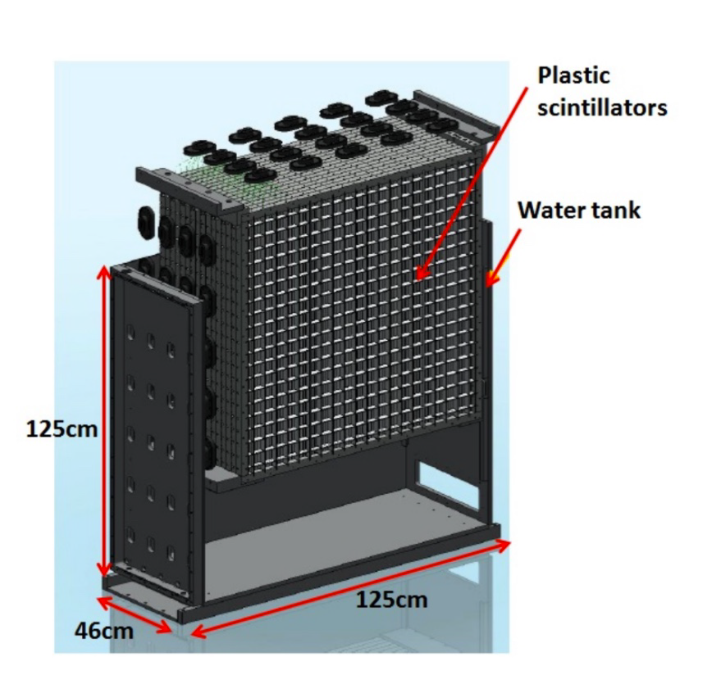
\includegraphics[width=\textwidth]{images/wagasci}
\end{column}
\begin{column}{.5\textwidth}
\begin{itemize}
\item Measure CC cross section ratio water/hydrocarbon with 3\% uncertainty
\item Measure CC cross section on water/hydrocarbon with large angular acceptance.
\end{itemize}

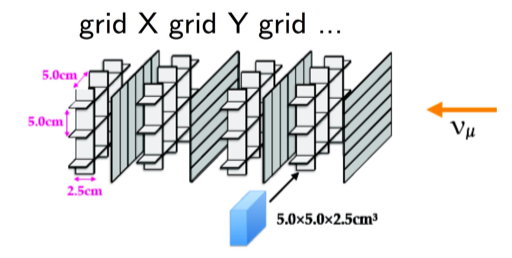
\includegraphics[width=\textwidth]{images/wagsche}
\end{column}
\end{columns}

\end{frame}

\begin{frame}{Topology}

\begin{columns}[c]
\begin{column}{.5\textwidth}
\begin{itemize}
    \item CC0$\pi^{+/-}$ is the signal (have no sensitivity to $\pi^0$ in WAGASCI) 
    \item Any event which produces one $\mu$, 0 $\pi$, any no. of photons in FS
    \item Where interaction happened in fiducial volume of detector
\end{itemize}
\end{column}
\begin{column}{.5\textwidth}
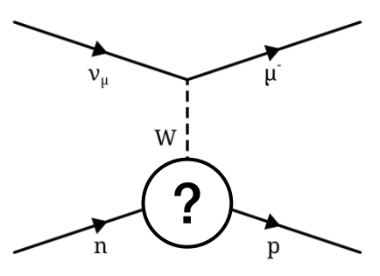
\includegraphics[width=\textwidth]{images/topology.png}
\end{column}
\end{columns}
\end{frame}

\begin{frame}{MC Simulation Description} 	

\begin{columns}
\begin{column}{.5\textwidth}
\begin{itemize}
	\item GEANT4 simulation of WAGASCI+Proton module+SideMRDs+BabyMIND
	\item Uses Neut file as input, interactions in scint. or water
	\item Accurate geometry and magnetic field description
	\item Output is ROOT Ntuple
	\item Separate package for populating recon track object  
\end{itemize}
\end{column}
\begin{column}{.5\textwidth}
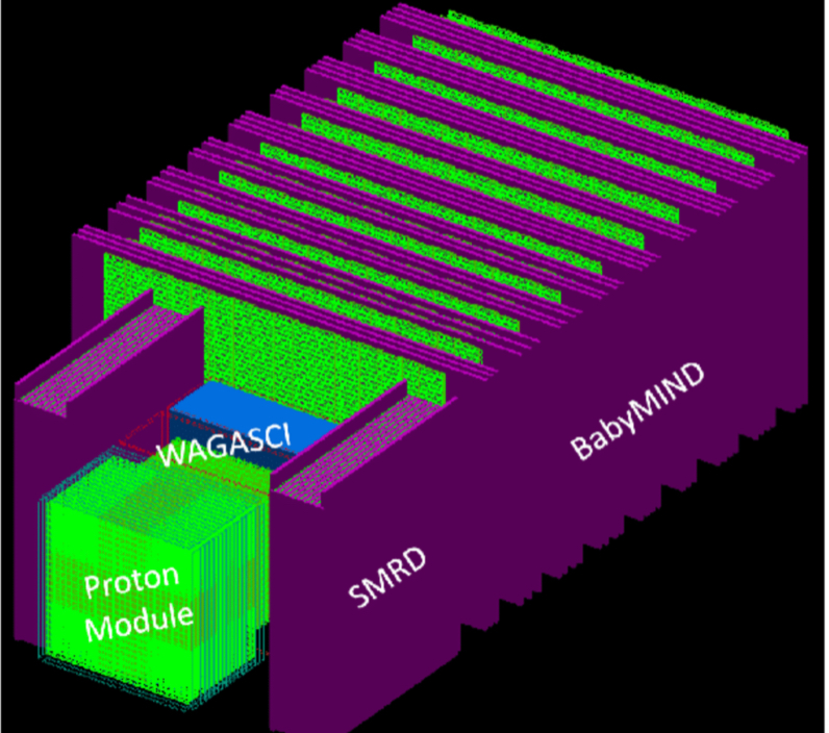
\includegraphics[width=\textwidth]{images/geo.pdf}
\end{column}	
\end{columns}

\end{frame}

\begin{frame}{WAGASCI software harmonisation}
    \begin{itemize}
        \item Several different packages
        \item No common install tool
        \item Some of current experts are now employed outside of T2K,  danger of losing institutional knowledge
        \item Many dependencies, difficult to keep track
        \item Many different versions of software also difficult to keep track
        \item Complex interdependency between packages
    \end{itemize}
\end{frame}

\begin{frame}{WAGASCI software harmonisation}
    \begin{itemize}
        \item WAGASCI MC: Main simulation package, GEANT4 simulation of B2 floor. All detectors, all fields, clustering, digitisation
        \begin{itemize}
            \item Dependencies: BOOST, ROOT, GEANT (Has installation script, git documentation)
        \end{itemize}
        \item WAGASCI Event Display: input is WAGASCI MC, output is image of detector with track overlaid
        \begin{itemize}
            \item Dependencies: WAGASCI MC (No installation script, git documentation)
        \end{itemize}
        \item WAGASCI Track Reconstruction: input is WAGASCI MC, output is file with recon branches filled, runs Kalman Filter
        \begin{itemize}
            \item Dependencies: Event Display, WAGASCI MC, GenFit: Eigen (No installation script, limited documentation, much of code still in development)
        \end{itemize}
        \item WAGASCIReWeight: input is WAGASCI MC, output is file with weight branches filled
        \begin{itemize}
            \item Dependencies: WAGASCI MC, T2KReWeight, NIWGReWeight, NEUT (No installation script, limited documentation, much of code still in development)
        \end{itemize}
    \end{itemize}

\end{frame}

\begin{frame}{WAGASCI software harmonisation}
    \begin{itemize}
        \item These package are built sequentially
        \item Later packages depend on earlier packages
        \item Dependencies, installation and ease of use..... calls for a container
        \item This software represents a huge amount of hard work by developers (Kenji, Giorgio and others) - do not want to lose this effort or tools
    \end{itemize}
\end{frame}

\begin{frame}{WAGASCI software harmonisation}

    \begin{itemize}
\item This is not sustainable
\item Difficult to reproduce problems
\item High entry barrier for new people
\item Contributing to framework non-trivial 
\item Solution: merge some of these projects
\item Just before Christmas created container for all WAGASCI software 
\item Packages remain separate and distinct allowing for parallel development but overall project can be accessed in one place and will run everywhere (in principle)
\item Added all packages, available from Docker Hub
\end{itemize}

\end{frame}

\begin{frame}{WAGASCI software harmonisation}
    \begin{itemize}
        \item Can go here: \url{https://hub.docker.com/r/jnugent42/wagasci_framework}
        \item Image contains all WAGASCI code
        \item No installation, no dependency hell
    \end{itemize}
    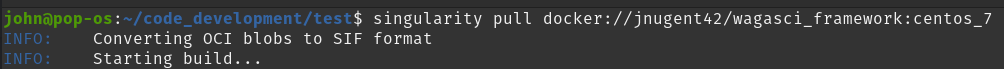
\includegraphics[width=\textwidth]{images/Screenshot from 2023-01-23 11-11-52.png}
\end{frame}

\begin{frame}{WAGASCI software harmonisation}
    \begin{itemize}
        \item Can run immediately
        \item Runs on any platform
        \item All packages in single image
        \item Image built from latest software branches on T2K GitLab: https://git.t2k.org/
    \end{itemize}
        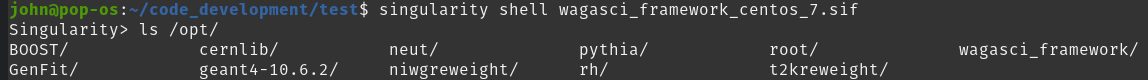
\includegraphics[width=\textwidth]{images/Screenshot from 2023-01-23 11-13-35.png}
\end{frame}

\begin{frame}{Sample definitions: WAGASCI}

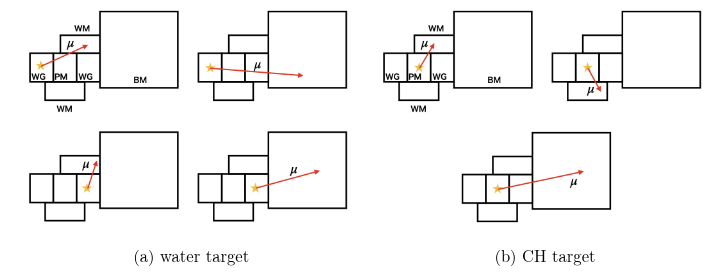
\includegraphics[width=\textwidth]{images/wag_sam.png}
\begin{itemize}
    \item Samples defined in TN455 for WAGASCI
    \item C$_8$H$_8$ target for WAGASCI 
    \item Also have large H$_2$0 target in WAGASCI \
    \item 7 WAGASCI samples 
\end{itemize}    
\vfill

\end{frame}

\begin{frame}{Sample definition: ND280}

\begin{columns}[c]
\begin{column}{.5\textwidth}
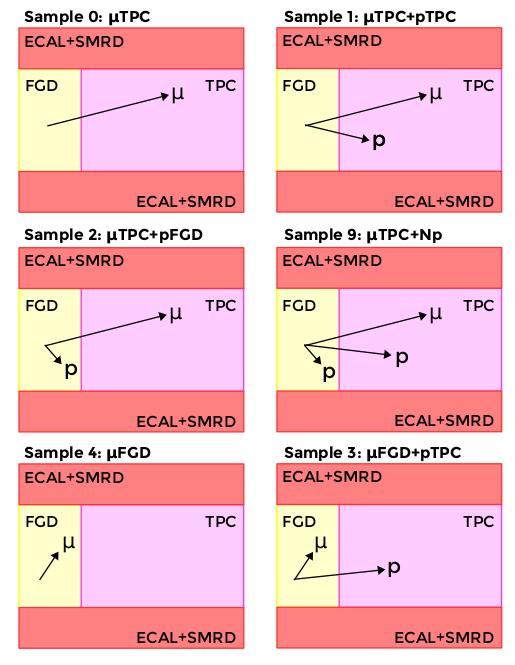
\includegraphics[width=\textwidth]{images/ND280_sig.png}
\end{column}
\begin{column}{.5\textwidth}
Both FGD1 and FGD2 samples are used 
\begin{itemize}
    \item $\mu$TPC 
    \item $\mu$TPC+pTPC
    \item $\mu$TPC+pFGD
    \item $\mu$TPC+Np
    \item $\mu$FGD 
    \item $\mu$FGD+pTPC 
\end{itemize}
\vfill
\begin{block}{}
\begin{itemize}
    \item Sideband available CC1$\pi$ sample \& sand muon sample WAGASCI
    \item Sideband available CC1$\pi$ sample \& CCother sample ND280
\end{itemize}
\end{block}
\end{column}
\end{columns}
\end{frame}

\begin{frame}{Current dataset}

\begin{columns}[c]
\begin{column}{.5\textwidth}
\begin{itemize}
    \item FHC ${\nu}_{\mu}$ mode 
    \item ND280 data on tape from Run 2, 3, 4, 8
    \item 11.52$\times10^{20}$ POT
    \item WAGASCI data on tape from Run 10 \& 11
    \item 6.55 $\times10^{20}$ POT
\end{itemize}    
\end{column}
\begin{column}{.5\textwidth}

\begin{table}[htp]
\begin{ruledtabular}
\begin{tabular}{c|c}
\hline
\hline 
Run & Data POT ($\times10^{20}$)\\
	\hline
 2 & 0.79 \\
 3 & 1.58 \\
 4 & 3.42 \\
8 & 5.73 \\
 10 & 2.65 \\
 11 & 3.90 \\ 
\hline
\hline 
\end{tabular}
\end{ruledtabular}
\end{table}

\end{column}
\end{columns}

\end{frame}

\begin{frame}{Code Versions}
\begin{itemize}
    \item ND280 software v13.14
    \item Highland v2.84.3
    \item numuCCZeroPi Master
    \item OA files from Grid 6AA production run 2, 3, 4 \& 8 (subset)
    \item No sand files
    \item \texttt{Neut\_D} MC files
    \item All plots are MC, no data files
    \item Written my own simple root macro to draw some plots with drawing tools
   \end{itemize}
\end{frame}

\begin{frame}{Question: Downloading ND280 MC+data}
    \begin{itemize}
        \item Previously had help from Sophie, still very much struggling 
        \item it has take of order ~1 month to download run4 MC
        \item still have several other sets that I want to use
    \end{itemize}
    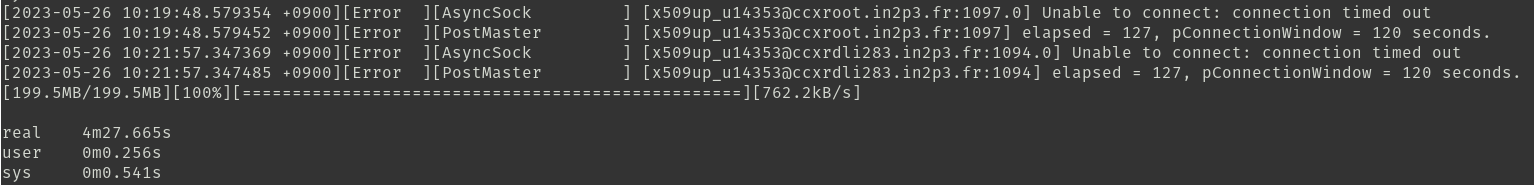
\includegraphics[width=\textwidth]{images/download_grid.png}
    \begin{itemize}
        \item \color{red}{Resolved: Using directory sync tools}
    \end{itemize}
\end{frame}

% \begin{frame}{Event Display: ND280}

% \vfill
% \begin{block}{}
% \begin{itemize}
%     \item Need to download recon files
% \end{itemize}
% \end{block}
% \end{frame}

% \begin{frame}{Event Display: WAGASCI}

% \vfill
% \begin{block}{}
% \begin{itemize}
%     \item Sideband available CC1$\pi$ sample 
%  \end{itemize}
% \end{block}
% \end{frame}

\begin{frame}{Phase space restrictions \& binning}

\begin{itemize}
    \item True $\mu$ angle $\leq$70$^\circ$
    \item True $\mu$ momentum $\geq$300 MeV/c
    \item Binning same as current WAGASCI analysis, WAGASCI data set is the limiting factor in terms of stats
    \item Will involve changing for ND280 but only reducing so straightforward : \color{red}{Done}
\end{itemize}    
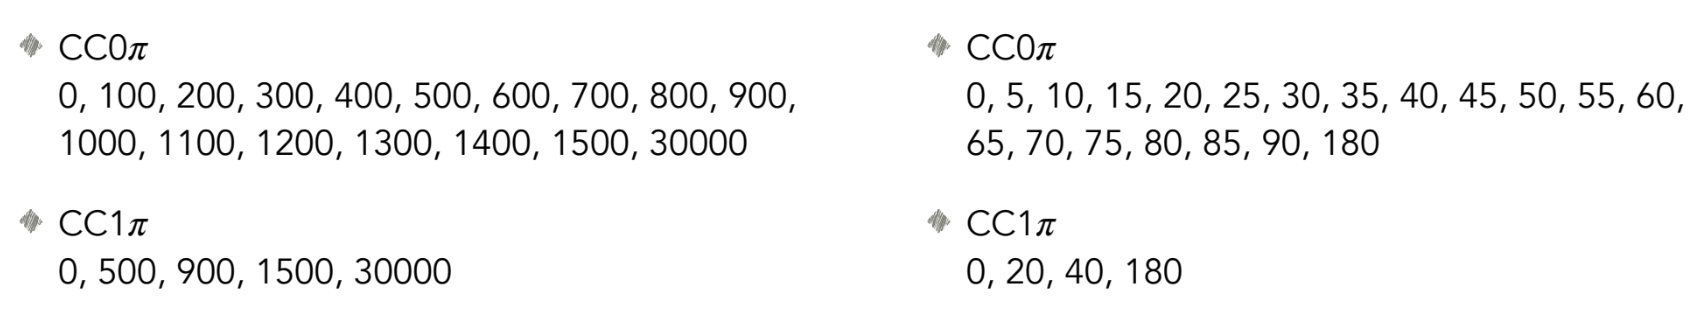
\includegraphics[width=\textwidth]{images/binning.png}
\end{frame}

\begin{frame}{C and H$_2$O Samples}
    \begin{itemize}
        \item Defined in the sample way as TN338
        \item FGD1 is C sample
        \item FGD2 has two samples; a C rich sample from the $y$ layer and a H$_2$O rich sample from the $x$ layer 
            \end{itemize}
            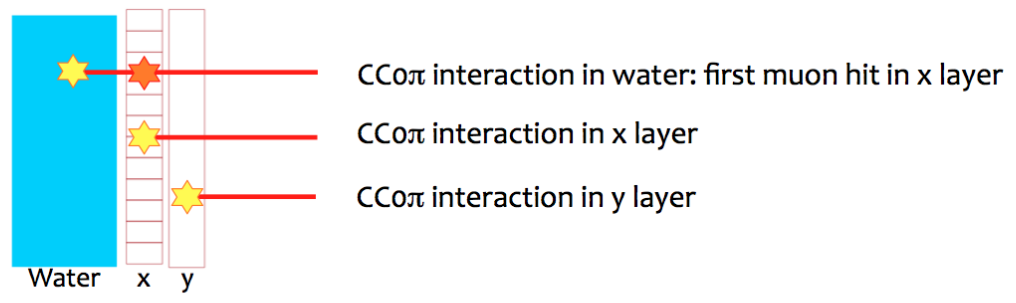
\includegraphics[width=\textwidth]{images/FGD2Layers.png}
\end{frame}

\begin{frame}{Selection}
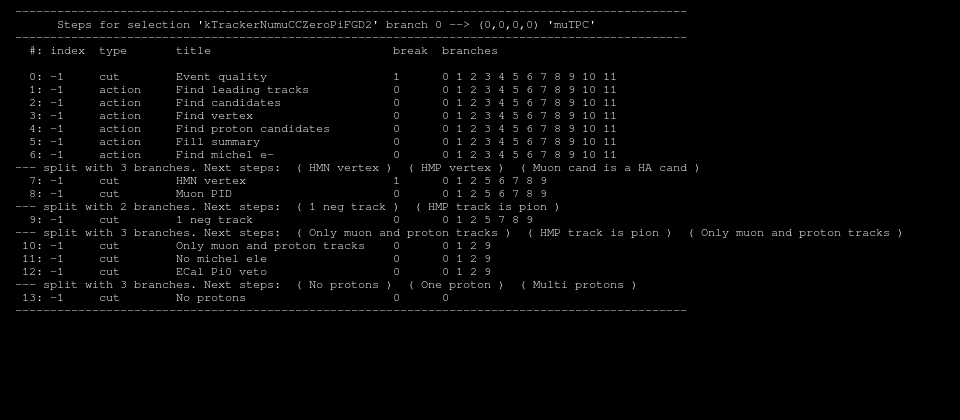
\includegraphics[width=\textwidth]{images/branch0.png}
\end{frame}
\begin{frame}{muTPC}
\center
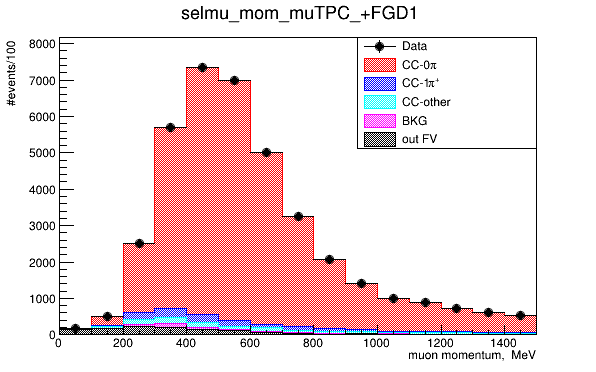
\includegraphics[width=.45\textwidth]{images/selmu_mom_topology_muTPC_accum_level[][0][07]_data_mc.png}
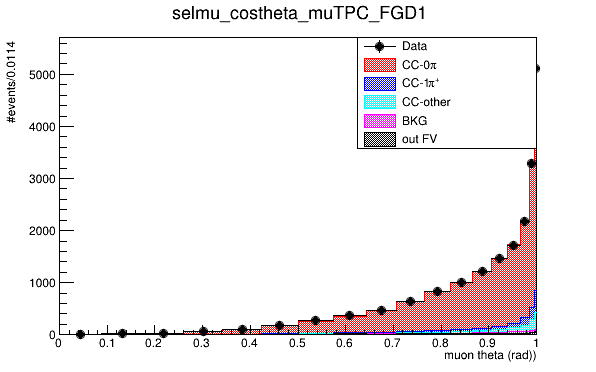
\includegraphics[width=.45\textwidth]{images/selmu_costheta_topology_muTPC_accum_level[][0][07]_data_mc.png}
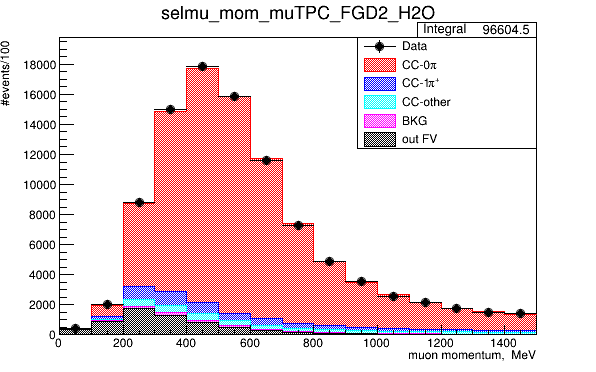
\includegraphics[width=.45\textwidth]{images/selmu_mom_fgd2topology_muTPC_accum_level[][1][07] && sample_fgd2layer_xsec==0_data_mc.png}
 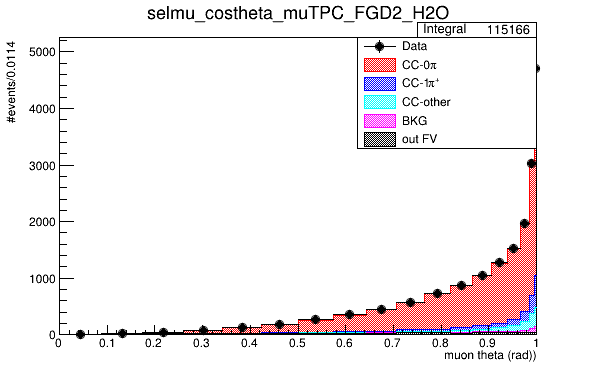
\includegraphics[width=.45\textwidth]{images/selmu_costheta_fgd2topology_muTPC_accum_level[][1][07] && sample_fgd2layer_xsec==0_data_mc.png}
 \end{frame}
\begin{frame}{muTPC}
\center
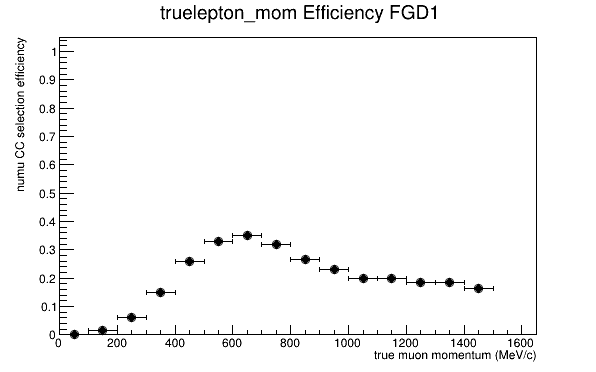
\includegraphics[width=.45\textwidth]{images/Eff_truelepton_mom_topology_muTPC_accum_level[][0][07]_data_mc.png}
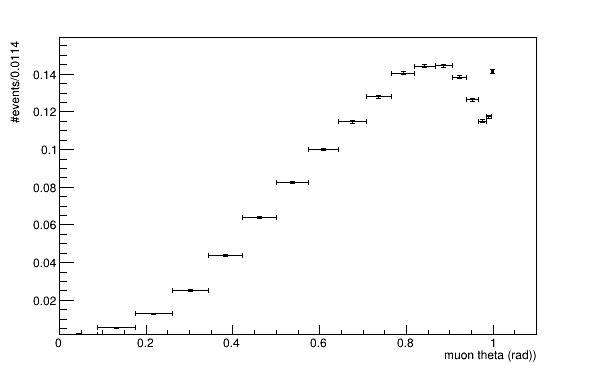
\includegraphics[width=.45\textwidth]{images/Eff_truelepton_costheta_topology_muTPC_accum_level[][0][07]_data_mc.png}
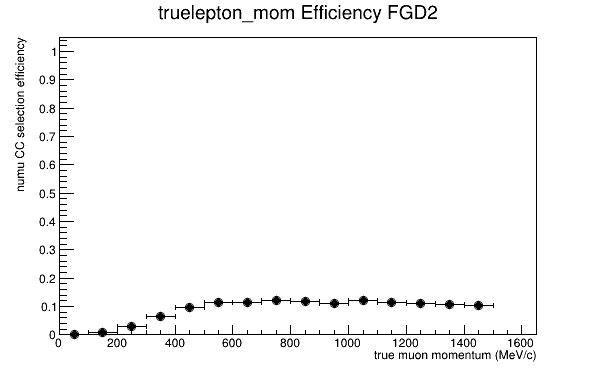
\includegraphics[width=.45\textwidth]{images/Eff_truelepton_mom_fgd2topology_muTPC_accum_level[][1][07]_data_mc.png}
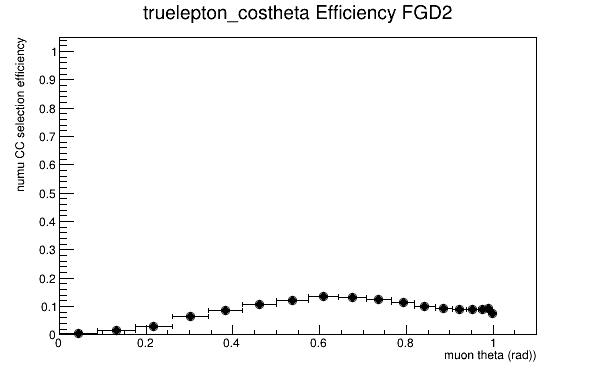
\includegraphics[width=.45\textwidth]{images/Eff_truelepton_costheta_fgd2topology_muTPC_accum_level[][1][07]_data_mc.png}
\end{frame}
\begin{frame}{muTPC}
\center
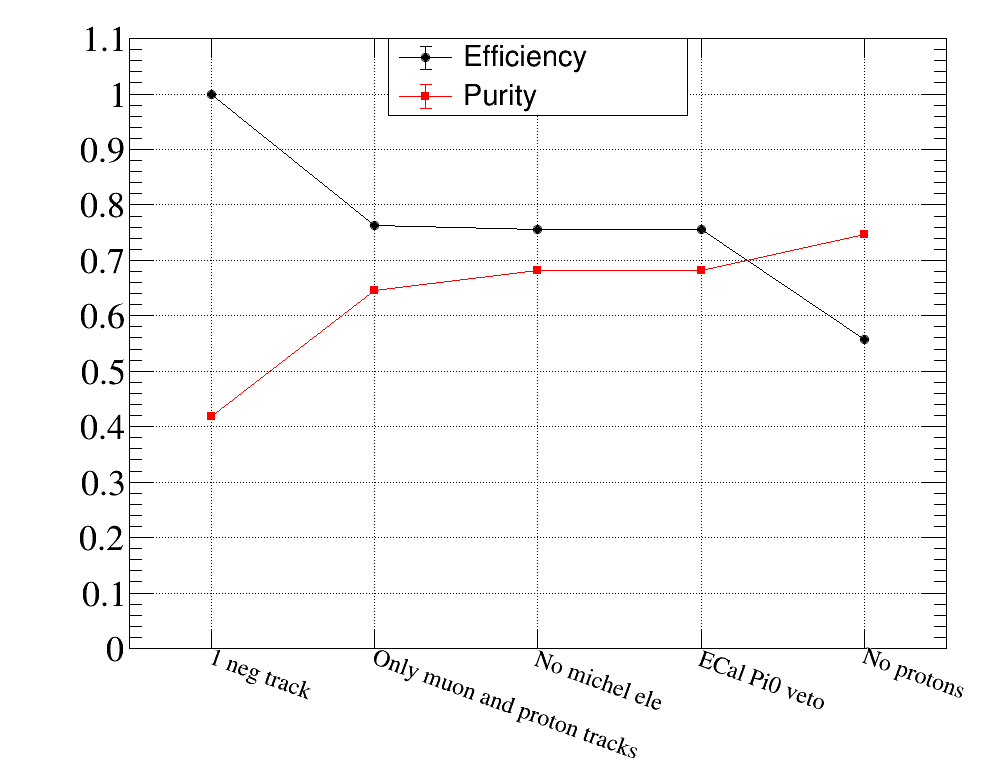
\includegraphics[width=.45\textwidth]{images/EffPurVsCut_br0_reaction.png}
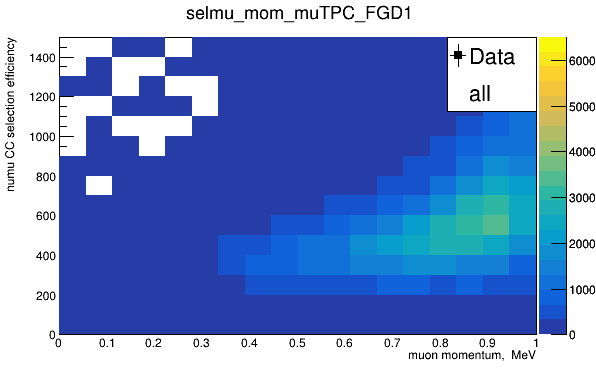
\includegraphics[width=.45\textwidth]{images/2D_selmu_mom:selmu_costheta_fgd2topology_muTPC_accum_level[][0][07]_data_mc.png}
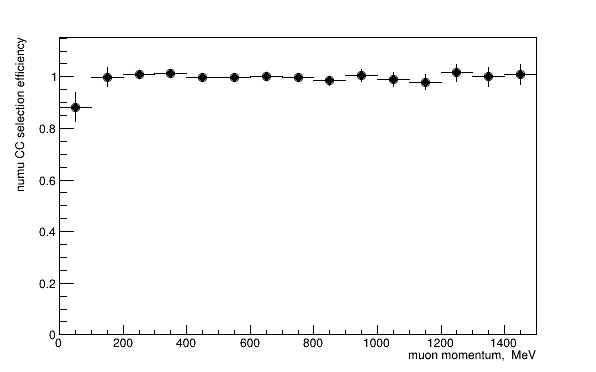
\includegraphics[width=.45\textwidth]{images/ratio_selmu_mom_topology_muTPC_accum_level[][0][07]_data_mc.png}
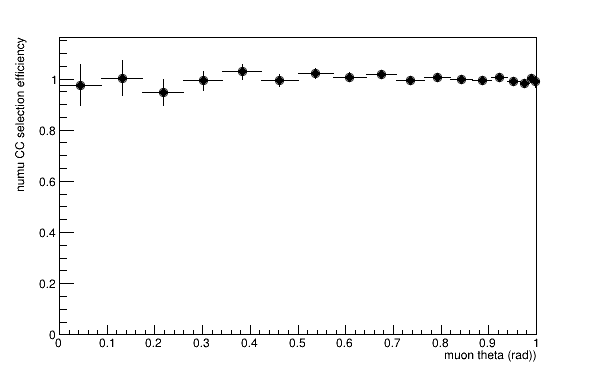
\includegraphics[width=.45\textwidth]{images/ratio_selmu_costheta_topology_muTPC_accum_level[][0][07]_data_mc.png}
\end{frame}

\begin{frame}{Takeaways}

\begin{itemize}
    \item 16 samples in total, plots for each sample (see backups)
    \item Have first pass of running ND280 selection out of the box
    \item Don't expect to much development on this side in this analysis, ND280 already well developed
    \item Plots are for my own reference
    \item I now have some familiarity with Highland, want to make same plots for WAGASCI 
    \item First sample selected for WAGASCI in Highland
\end{itemize}

\end{frame}

\begin{frame}{Code Versions}
\begin{itemize}
    \item ND280 software v13.14
    \item Highland v2.84.3
    \item wgbmNuMuCC0Pi\_highland\_integration
    \item Ran WGMC$\rightarrow$WGTR to produce WG files 
    \item All plots are MC, no data files
    \item Written my own simple root macro to draw some plots with drawing tools 
\end{itemize}
 \begin{itemize}
       \item \color{red} Want to run larger jobs over more MC and data files. Currently takes very long time. Not unexpected using large files. Investigate WAGASCI file structure.
   \end{itemize}
\end{frame}

\begin{frame}{Vertex}
    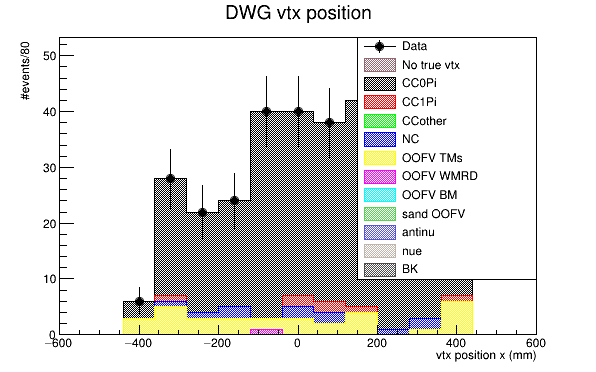
\includegraphics[width=0.45\textwidth]{images/vtx_reco_pos[0]_wgbm_topo_DWG_accum_level[][26]_data_mc.png}
    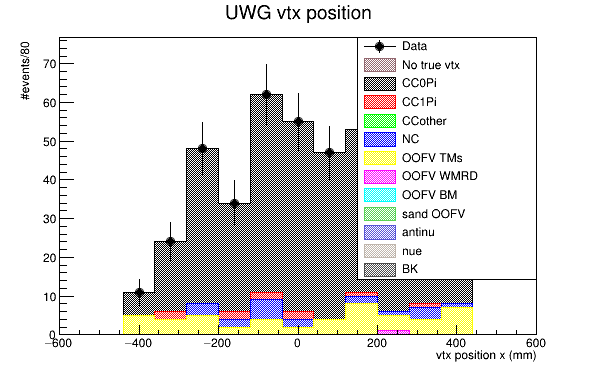
\includegraphics[width=0.45\textwidth]{images/vtx_reco_pos[0]_wgbm_topo_UWG_accum_level[][16]_data_mc.png}
    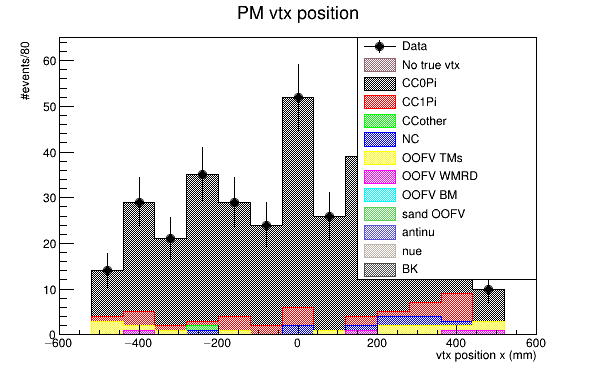
\includegraphics[width=0.45\textwidth]{images/vtx_reco_pos[0]_wgbm_topo_PM_accum_level[][06]_data_mc.png}
\end{frame}

\begin{frame}{Vertex}
    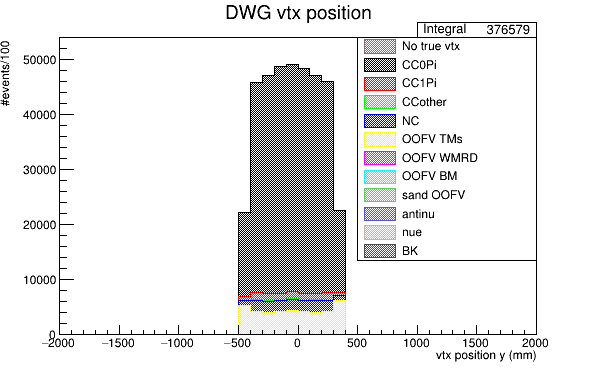
\includegraphics[width=0.45\textwidth]{images/vtx_reco_pos[1]_wgbm_topo_DWG_accum_level[][26]_data_mc.png}
    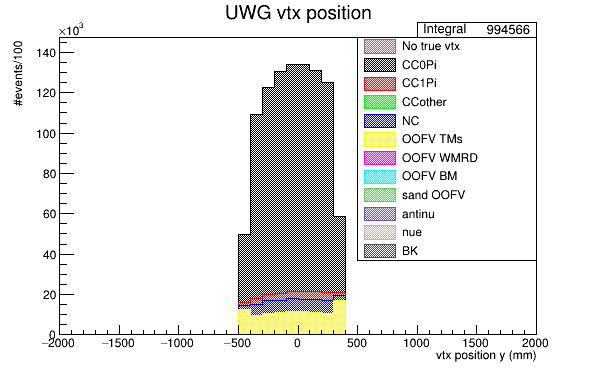
\includegraphics[width=0.45\textwidth]{images/vtx_reco_pos[1]_wgbm_topo_UWG_accum_level[][16]_data_mc.png}
    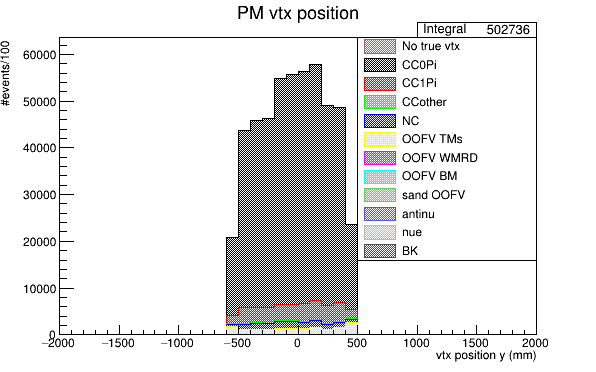
\includegraphics[width=0.45\textwidth]{images/vtx_reco_pos[1]_wgbm_topo_PM_accum_level[][06]_data_mc.png}
\end{frame}

\begin{frame}{Vertex}
    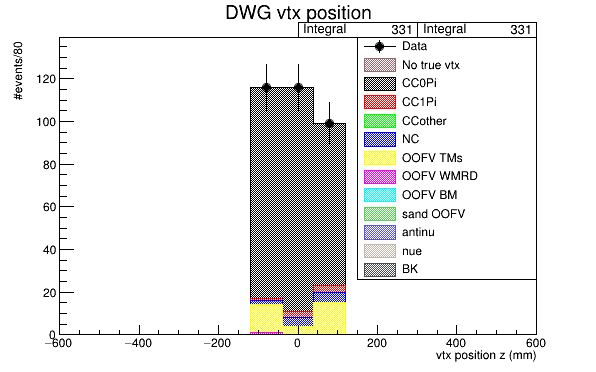
\includegraphics[width=0.45\textwidth]{images/vtx_reco_pos[2]_wgbm_topo_DWG_accum_level[][26]_data_mc.png}
    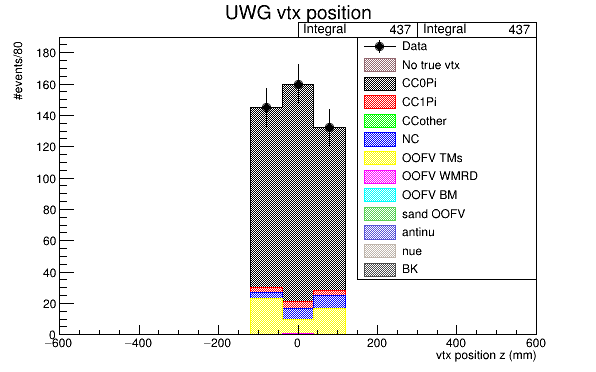
\includegraphics[width=0.45\textwidth]{images/vtx_reco_pos[2]_wgbm_topo_UWG_accum_level[][16]_data_mc.png}
    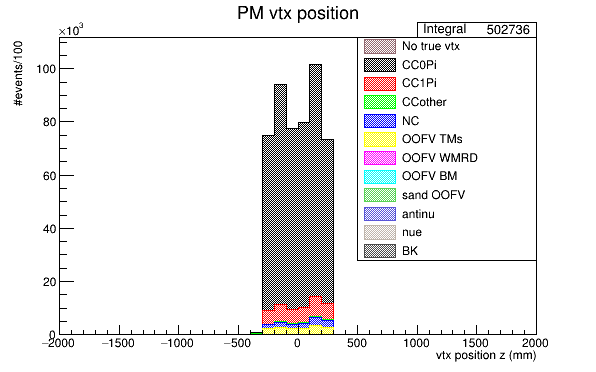
\includegraphics[width=0.45\textwidth]{images/vtx_reco_pos[2]_wgbm_topo_PM_accum_level[][06]_data_mc.png}
\end{frame}

\begin{frame}{No. of tracks}
    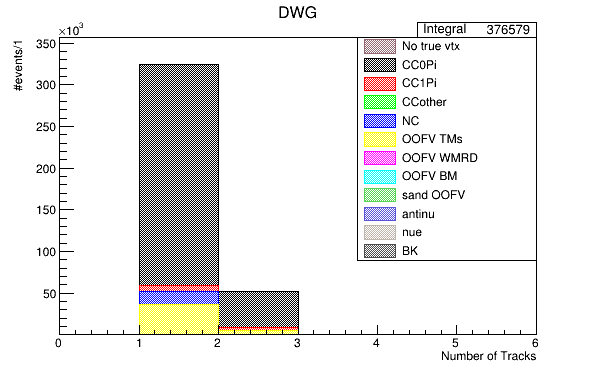
\includegraphics[width=0.45\textwidth]{images/num_of_vtx_reco_tracks_wgbm_topo_DWG_accum_level[][26]_data_mc.png}
    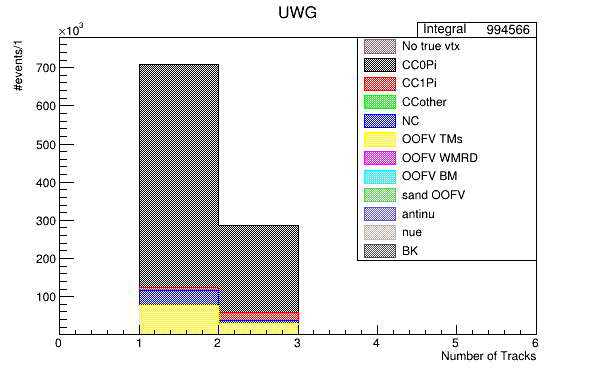
\includegraphics[width=0.45\textwidth]{images/num_of_vtx_reco_tracks_wgbm_topo_UWG_accum_level[][16]_data_mc.png}
    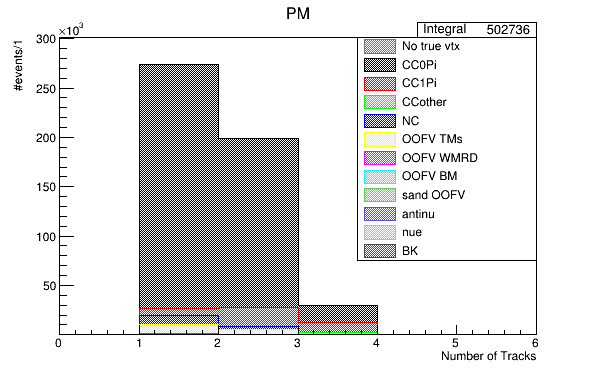
\includegraphics[width=0.45\textwidth]{images/num_of_vtx_reco_tracks_wgbm_topo_PM_accum_level[][06]_data_mc.png}
\end{frame}

\begin{frame}{$\mu$ CL}
    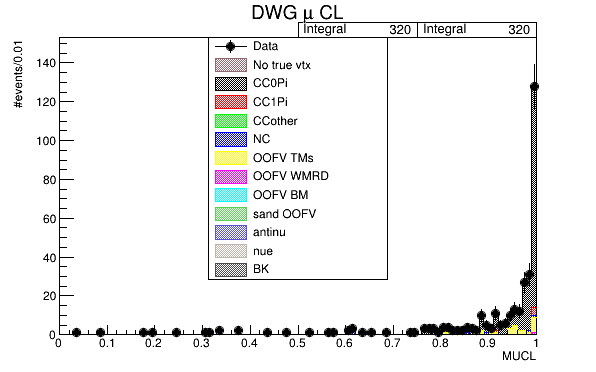
\includegraphics[width=0.45\textwidth]{images/mucl_dwg_wgbm_topo_DWG_accum_level[][26]_data_mc.png}
    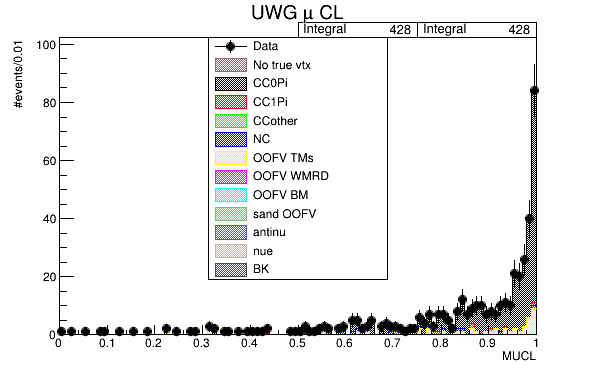
\includegraphics[width=0.45\textwidth]{images/mucl_uwg_wgbm_topo_UWG_accum_level[][16]_data_mc.png}
    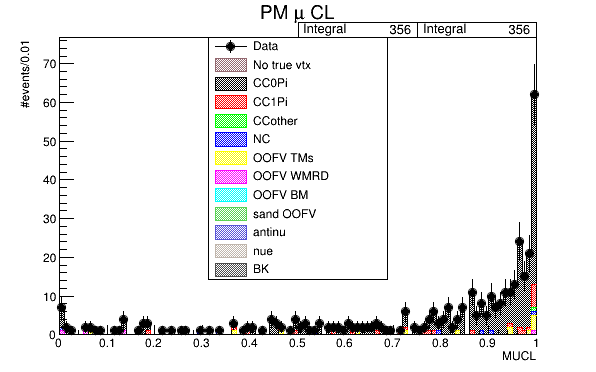
\includegraphics[width=0.45\textwidth]{images/mucl_pm_wgbm_topo_PM_accum_level[][06]_data_mc.png}
\end{frame}

\begin{frame}{Charge -ve}
    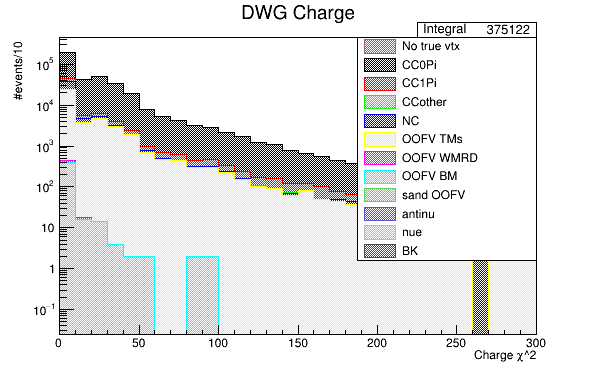
\includegraphics[width=0.45\textwidth]{images/charge_neg_chi2_wgbm_topo_DWG_accum_level[][26]_data_mc.png}
    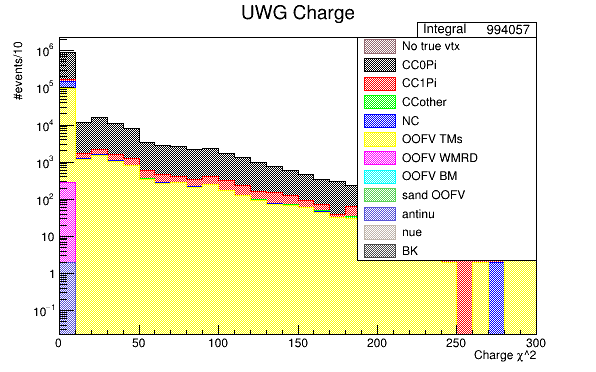
\includegraphics[width=0.45\textwidth]{images/charge_neg_chi2_wgbm_topo_UWG_accum_level[][16]_data_mc.png}
    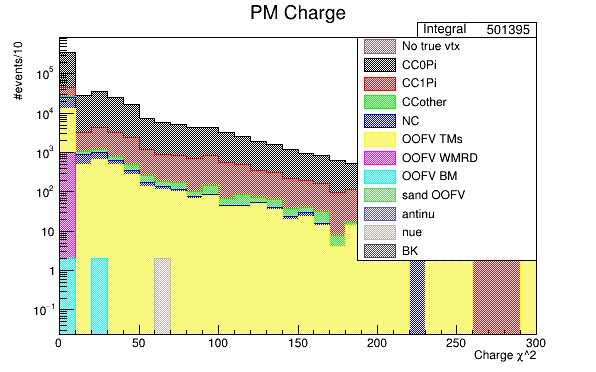
\includegraphics[width=0.45\textwidth]{images/charge_neg_chi2_wgbm_topo_PM_accum_level[][06]_data_mc.png}
\end{frame}

\begin{frame}{Charge +ve}
    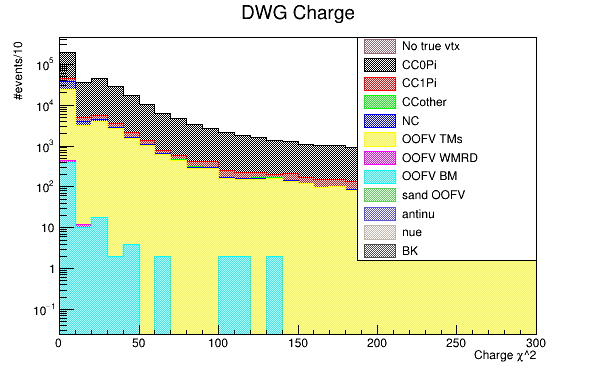
\includegraphics[width=0.45\textwidth]{images/charge_pos_chi2_wgbm_topo_DWG_accum_level[][26]_data_mc.png}
    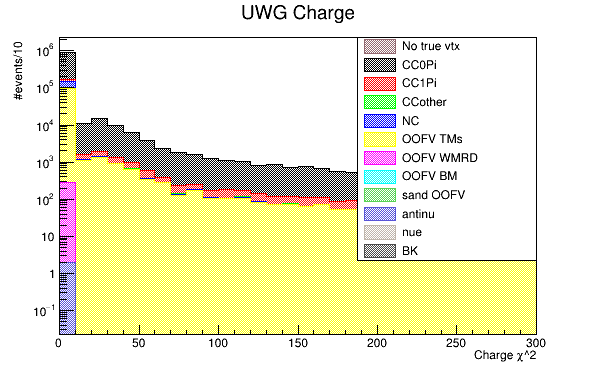
\includegraphics[width=0.45\textwidth]{images/charge_pos_chi2_wgbm_topo_UWG_accum_level[][16]_data_mc.png}
    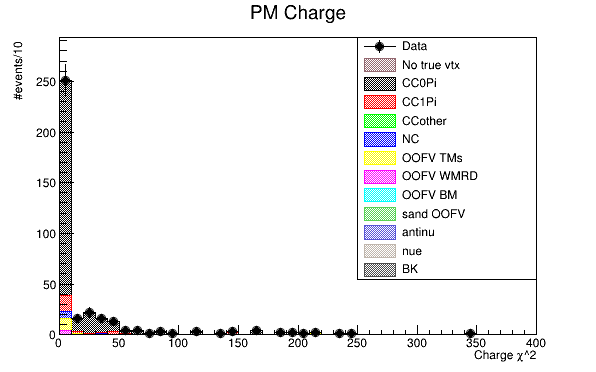
\includegraphics[width=0.45\textwidth]{images/charge_pos_chi2_wgbm_topo_PM_accum_level[][06]_data_mc.png}
\end{frame}

\begin{frame}{Track to cluster ratio}
    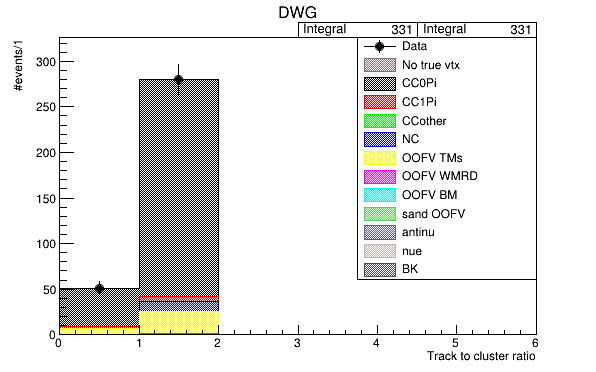
\includegraphics[width=0.45\textwidth]{images/track_to_cluster_hits_ratio_wgbm_topo_DWG_accum_level[][26]_data_mc.png}
    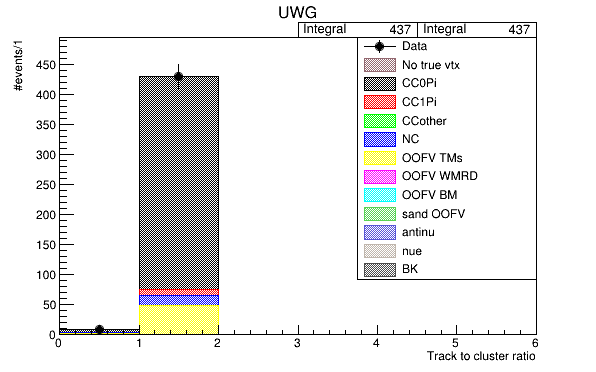
\includegraphics[width=0.45\textwidth]{images/track_to_cluster_hits_ratio_wgbm_topo_UWG_accum_level[][16]_data_mc.png}
    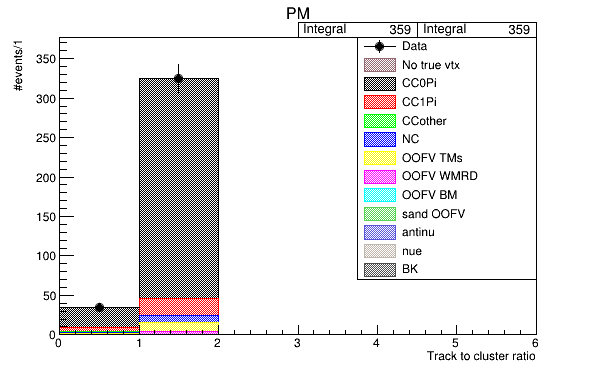
\includegraphics[width=0.45\textwidth]{images/track_to_cluster_hits_ratio_wgbm_topo_PM_accum_level[][06]_data_mc.png}
\end{frame}

\begin{frame}{No. of delayed hits}
    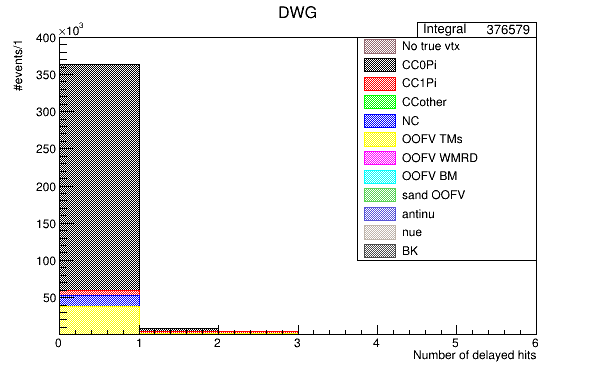
\includegraphics[width=0.45\textwidth]{images/num_reco_delayed_hits_wgbm_topo_DWG_accum_level[][26]_data_mc.png}
    \includegraphics[width=0.45\textwidth]{images/num_reco_delayed_hits_wgbm_topo_UWG_accum_level[][16]_data_mc.png}
    \includegraphics[width=0.45\textwidth]{images/num_reco_delayed_hits_wgbm_topo_PM_accum_level[][06]_data_mc.png}
\end{frame}

\begin{frame}{Selection}
\includegraphics[width=\textwidth]{images/branch0.png}
\end{frame}
\begin{frame}{PM}
\center
\includegraphics[width=.45\textwidth]{images/selmu_reco_mom_range_PM_wgbm_topo_accum_level[][06]_data_mc.png}
\includegraphics[width=.45\textwidth]{images/selmu_reco_costheta_wgbm_topo_PM_accum_level[][06]_data_mc.png}
\end{frame}
\begin{frame}{PM}
\center
\includegraphics[width=.45\textwidth]{images/Eff_selmu_true_mom_wgbm_topo_PM_accum_level[][06]_data_mc.png}
\includegraphics[width=.45\textwidth]{images/Eff_selmu_true_costheta_wgbm_topo_PM_accum_level[][06]_data_mc.png}
\end{frame}
\begin{frame}{PM}
\center
\includegraphics[width=.45\textwidth]{images/EffPurVsCut_br0_true_wgbm_topo.png}
\includegraphics[width=.45\textwidth]{images/2D_selmu_mom:selmu_costheta_wgbm_topo_accum_level[][06]_data_mc.png}
\includegraphics[width=.45\textwidth]{images/ratio_selmu_reco_mom_range_wgbm_topo_accum_level[][06]_data_mc.png}
\includegraphics[width=.45\textwidth]{images/ratio_selmu_reco_costheta_wgbm_topo_PM_accum_level[][06]_data_mc.png}
\end{frame}
\begin{frame}{Selection}
\includegraphics[width=\textwidth]{images/branch1.png}
\end{frame}
\begin{frame}{UWG}
\center
\includegraphics[width=.45\textwidth]{images/selmu_reco_mom_range_UWG_wgbm_topo_accum_level[][16]_data_mc.png}
\includegraphics[width=.45\textwidth]{images/selmu_reco_costheta_wgbm_topo_UWG_accum_level[][16]_data_mc.png}
\end{frame}
\begin{frame}{UWG}
\center
\includegraphics[width=.45\textwidth]{images/Eff_selmu_true_mom_wgbm_topo_UWG_accum_level[][16]_data_mc.png}
\includegraphics[width=.45\textwidth]{images/Eff_selmu_true_costheta_wgbm_topo_UWG_accum_level[][16]_data_mc.png}
\end{frame}
\begin{frame}{UWG}
\center
\includegraphics[width=.45\textwidth]{images/EffPurVsCut_br1_true_wgbm_topo.png}
\includegraphics[width=.45\textwidth]{images/2D_selmu_mom:selmu_costheta_wgbm_topo_accum_level[][16]_data_mc.png}
\includegraphics[width=.45\textwidth]{images/ratio_selmu_reco_mom_range_wgbm_topo_accum_level[][16]_data_mc.png}
\includegraphics[width=.45\textwidth]{images/ratio_selmu_reco_costheta_wgbm_topo_UWG_accum_level[][16]_data_mc.png}
\end{frame}
\begin{frame}{Selection}
\includegraphics[width=\textwidth]{images/branch2.png}
\end{frame}
\begin{frame}{DWG}
\center
\includegraphics[width=.45\textwidth]{images/selmu_reco_mom_range_DWG_wgbm_topo_accum_level[][26]_data_mc.png}
\includegraphics[width=.45\textwidth]{images/selmu_reco_costheta_wgbm_topo_DWG_accum_level[][26]_data_mc.png}
\end{frame}
\begin{frame}{DWG}
\center
\includegraphics[width=.45\textwidth]{images/Eff_selmu_true_mom_wgbm_topo_DWG_accum_level[][26]_data_mc.png}
\includegraphics[width=.45\textwidth]{images/Eff_selmu_true_costheta_wgbm_topo_DWG_accum_level[][26]_data_mc.png}
\end{frame}
\begin{frame}{DWG}
\center
\includegraphics[width=.45\textwidth]{images/EffPurVsCut_br2_true_wgbm_topo.png}
\includegraphics[width=.45\textwidth]{images/2D_selmu_mom:selmu_costheta_wgbm_topo_accum_level[][26]_data_mc.png}
\includegraphics[width=.45\textwidth]{images/ratio_selmu_reco_mom_range_wgbm_topo_accum_level[][26]_data_mc.png}
\includegraphics[width=.45\textwidth]{images/ratio_selmu_reco_costheta_wgbm_topo_DWG_accum_level[][26]_data_mc.png}
\end{frame}

\begin{frame}{Optimise selection}

\begin{itemize}
    \item Can reuse selections as defined currently for ND280 \& WAGASCI
    \item Already published, reasonable samples with good purity \& efficiencies
    \item Improvements can be made, particularly on the WAGASCI side - optimisation of cut values
    \item I had already suggested this when doing the review of the TN for the current analysis
    \item Implementation of machine learning would take significantly longer and may not be feasible
    \item Current selection already in health state
    \item Priority: \color{red} Low
\end{itemize}
\end{frame}

% \begin{frame}{Question: Efficiencies for WAGASCI}
%     \begin{itemize}
%     \item Many errors when calculating efficiencies
%     \begin{itemize}
%         \item More events selected than in topology, probably tagging issue
%         \item in truth tree all topologies are -999
%     \end{itemize}
%         \item Efficiencies for WAGASCI are very small ~0.001\%
%         \item Can trace this behaviour to the large no. of truth events
%         \item there are two behaviours here:
%         \begin{itemize}
%            \item due to the way in which the FV selection is currently defined
%         \item Also only have one `tag' for events \texttt{wgbm\_topo}, need other such as \texttt{reaction==} $\rightarrow$ in progress
%         \item \textcolor{red}{Discussed with Cesar: may just be DrawingTools issue}
%         \end{itemize}
%     \end{itemize}
%         \includegraphics[width=.45\textwidth]{images/hmc1.png}
%         \includegraphics[width=.45\textwidth]{images/hmc2.png}
% \end{frame}

\begin{frame}{eff \& pur for all cuts bar one}
    \begin{itemize}
        \item Want to study impact of one individual cut, turn off only that cut
        \item Thanks for Nick who made a script which does this job available, have adapted for WAGASCI
    \end{itemize}
    \center
    \includegraphics[width=.45\textwidth]{images/nMinusOneCuts_sample2.png}
    \includegraphics[width=.45\textwidth]{images/nMinusOneCuts_sample1.png}
    \includegraphics[width=.45\textwidth]{images/nMinusOneCuts_sample0.png}
\end{frame}

\begin{frame}{NEUTgeom}
    \begin{itemize}
        \item Current NEUT implementation for WAGASCI not optimised
        \item NEUT is run seperately for each target, i.e., UWG, DWG, BM, WMS, etc......
        \item Each Wall (sand) event is given an increased weight due to low stats in this sample
        \item Results in some very large weights for individual Wall (sand) events, resulting distributions aesthetically unpleasing
        \item Avoid this issue by generating event in same way as ND280, NEUTgeom
        \item One simulation, each material in geometry gets own events from NEUT
        \item Developing code to make first pass of this now
    \end{itemize}
\end{frame}

\begin{frame}{JPARC activity}
\includegraphics[width=.3\textwidth]{images/IMG_2161.jpg}
%\includegraphics[width=.4\textwidth]{Group Meeting Kalman/images/IMG02444_HDR.jpg}
%\includegraphics[width=.4\textwidth]{Group Meeting Kalman/images/WAG_moreside.png}
\includegraphics[width=.3\textwidth]{images/water_tank.jpg}
\includegraphics[width=.3\textwidth]{images/IMG02444_HDR.jpg}
    \begin{itemize}
            \item In December 2022 spent 2 weeks at J-PARC with Arihara-san and Honjo-san prepping the detector for beam, i.e., filling the water modules, calibrating the detector, shaking down hardware
            \item June 2023 spent 2 weeks at J-PARC turning on detector calibrating each module, minor repair work, prep for beam
            \item WAGASCI is in desperate need of more person power 
            \end{itemize}
\end{frame}

\begin{frame}{Next steps}

\begin{itemize}
    \item First pass of running ND280 selection (for me) 
    \item First pass of running WAGASCI selection (in highland)
\end{itemize}
\begin{itemize}
    \item Finalise selection for analysis \cmark
    \item download more MC+data to run with \cmark
    \item Finish tidying up plots and run with more stats
    \begin{itemize}
        \item ND280 can run larger stat MC plots \cmark
        \item ND280 can run larger stat MC+data plots \cmark
        \item WAGASCI can run larger stat MC plots \cmark
        \item WAGASCI can run larger stat MC+data plots \xmark
    \end{itemize}
    \item Implement NEUTgeom
\end{itemize}
    
\end{frame}

\appendix

\begin{frame}{Highland Corrections}
\includegraphics[width=\textwidth]{images/corrections.png}
\end{frame}

\begin{frame}{Selection}
\includegraphics[width=\textwidth]{images/branch1.png}
\end{frame}
\begin{frame}{muTPC+pTPC}
\center
\includegraphics[width=.45\textwidth]{images/selmu_mom_topology_muTPC+pTPC_accum_level[][0][18]_data_mc.png}
\includegraphics[width=.45\textwidth]{images/selmu_costheta_topology_muTPC+pTPC_accum_level[][0][18]_data_mc.png}
\includegraphics[width=.45\textwidth]{images/selmu_mom_fgd2topology_muTPC+pTPC_accum_level[][1][18]_data_mc.png}
\includegraphics[width=.45\textwidth]{images/selmu_costheta_fgd2topology_muTPC+pTPC_accum_level[][1][18]_data_mc.png}
\end{frame}
\begin{frame}{muTPC+pTPC}
\center
\includegraphics[width=.45\textwidth]{images/Eff_truelepton_mom_topology_muTPC+pTPC_accum_level[][0][18]_data_mc.png}
\includegraphics[width=.45\textwidth]{images/Eff_truelepton_costheta_topology_muTPC+pTPC_accum_level[][0][18]_data_mc.png}
\includegraphics[width=.45\textwidth]{images/Eff_truelepton_mom_fgd2topology_muTPC+pTPC_accum_level[][1][18]_data_mc.png}
\includegraphics[width=.45\textwidth]{images/Eff_truelepton_costheta_fgd2topology_muTPC+pTPC_accum_level[][1][18]_data_mc.png}
\end{frame}
\begin{frame}{muTPC+pTPC}
\center
\includegraphics[width=.45\textwidth]{images/muTPC+pTPC1_eff_pur_cut.png}
\includegraphics[width=.45\textwidth]{images/2D_selmu_mom:selmu_costheta_fgd2topology_muTPC+pTPC_accum_level[][0][18]_data_mc.png}
\includegraphics[width=.45\textwidth]{images/ratio_selmu_mom_topology_muTPC+pTPC_accum_level[][0][18]_data_mc.png}
\includegraphics[width=.45\textwidth]{images/ratio_selmu_costheta_topology_muTPC+pTPC_accum_level[][0][18]_data_mc.png}
\end{frame}
\begin{frame}{Selection}
\includegraphics[width=\textwidth]{images/branch2.png}
\end{frame}
\begin{frame}{muTPC+pFGD}
\center
\includegraphics[width=.45\textwidth]{images/selmu_mom_topology_muTPC+pFGD_accum_level[][0][29]_data_mc.png}
\includegraphics[width=.45\textwidth]{images/selmu_costheta_topology_muTPC+pFGD_accum_level[][0][29]_data_mc.png}
\includegraphics[width=.45\textwidth]{images/selmu_mom_fgd2topology_muTPC+pFGD_accum_level[][1][29]_data_mc.png}
\includegraphics[width=.45\textwidth]{images/selmu_costheta_fgd2topology_muTPC+pFGD_accum_level[][1][29]_data_mc.png}
\end{frame}
\begin{frame}{muTPC+pFGD}
\center
\includegraphics[width=.45\textwidth]{images/Eff_truelepton_mom_topology_muTPC+pFGD_accum_level[][0][29]_data_mc.png}
\includegraphics[width=.45\textwidth]{images/Eff_truelepton_costheta_topology_muTPC+pFGD_accum_level[][0][29]_data_mc.png}
\includegraphics[width=.45\textwidth]{images/Eff_truelepton_mom_fgd2topology_muTPC+pFGD_accum_level[][1][29]_data_mc.png}
\includegraphics[width=.45\textwidth]{images/Eff_truelepton_costheta_fgd2topology_muTPC+pFGD_accum_level[][1][29]_data_mc.png}
\end{frame}
\begin{frame}{muTPC+pFGD}
\center
\includegraphics[width=.45\textwidth]{images/muTPC+pFGD2_eff_pur_cut.png}
\includegraphics[width=.45\textwidth]{images/2D_selmu_mom:selmu_costheta_fgd2topology_muTPC+pFGD_accum_level[][0][29]_data_mc.png}
\includegraphics[width=.45\textwidth]{images/ratio_selmu_mom_topology_muTPC+pFGD_accum_level[][0][29]_data_mc.png}
\includegraphics[width=.45\textwidth]{images/ratio_selmu_costheta_topology_muTPC+pFGD_accum_level[][0][29]_data_mc.png}
\end{frame}
\begin{frame}{Selection}
\includegraphics[width=\textwidth]{images/branch3.png}
\end{frame}
\begin{frame}{muFGD+pTPC}
\center
\includegraphics[width=.45\textwidth]{images/selmu_mom_topology_muFGD+pTPC_accum_level[][0][310]_data_mc.png}
\includegraphics[width=.45\textwidth]{images/selmu_costheta_topology_muFGD+pTPC_accum_level[][0][310]_data_mc.png}
\includegraphics[width=.45\textwidth]{images/selmu_mom_fgd2topology_muFGD+pTPC_accum_level[][1][310]_data_mc.png}
\includegraphics[width=.45\textwidth]{images/selmu_costheta_fgd2topology_muFGD+pTPC_accum_level[][1][310]_data_mc.png}
\end{frame}
\begin{frame}{muFGD+pTPC}
\center
\includegraphics[width=.45\textwidth]{images/Eff_truelepton_mom_topology_muFGD+pTPC_accum_level[][0][310]_data_mc.png}
\includegraphics[width=.45\textwidth]{images/Eff_truelepton_costheta_topology_muFGD+pTPC_accum_level[][0][310]_data_mc.png}
\includegraphics[width=.45\textwidth]{images/Eff_truelepton_mom_fgd2topology_muFGD+pTPC_accum_level[][1][310]_data_mc.png}
\includegraphics[width=.45\textwidth]{images/Eff_truelepton_costheta_fgd2topology_muFGD+pTPC_accum_level[][1][310]_data_mc.png}
\end{frame}
\begin{frame}{muFGD+pTPC}
\center
\includegraphics[width=.45\textwidth]{images/muFGD+pTPC3_eff_pur_cut.png}
\includegraphics[width=.45\textwidth]{images/2D_selmu_mom:selmu_costheta_fgd2topology_muFGD+pTPC_accum_level[][0][310]_data_mc.png}
\includegraphics[width=.45\textwidth]{images/ratio_selmu_mom_topology_muFGD+pTPC_accum_level[][0][310]_data_mc.png}
\includegraphics[width=.45\textwidth]{images/ratio_selmu_costheta_topology_muFGD+pTPC_accum_level[][0][310]_data_mc.png}
\end{frame}
\begin{frame}{Selection}
\includegraphics[width=\textwidth]{images/branch4.png}
\end{frame}
\begin{frame}{muFGD}
\center
\includegraphics[width=.45\textwidth]{images/selmu_mom_topology_muFGD_accum_level[][0][49]_data_mc.png}
\includegraphics[width=.45\textwidth]{images/selmu_costheta_topology_muFGD_accum_level[][0][49]_data_mc.png}
\includegraphics[width=.45\textwidth]{images/selmu_mom_fgd2topology_muFGD_accum_level[][1][49]_data_mc.png}
\includegraphics[width=.45\textwidth]{images/selmu_costheta_fgd2topology_muFGD_accum_level[][1][49]_data_mc.png}
\end{frame}
\begin{frame}{muFGD}
\center
\includegraphics[width=.45\textwidth]{images/Eff_truelepton_mom_topology_muFGD_accum_level[][0][49]_data_mc.png}
\includegraphics[width=.45\textwidth]{images/Eff_truelepton_costheta_topology_muFGD_accum_level[][0][49]_data_mc.png}
\includegraphics[width=.45\textwidth]{images/Eff_truelepton_mom_fgd2topology_muFGD_accum_level[][1][49]_data_mc.png}
\includegraphics[width=.45\textwidth]{images/Eff_truelepton_costheta_fgd2topology_muFGD_accum_level[][1][49]_data_mc.png}
\end{frame}
\begin{frame}{muFGD}
\center
\includegraphics[width=.45\textwidth]{images/muFGD4_eff_pur_cut.png}
\includegraphics[width=.45\textwidth]{images/2D_selmu_mom:selmu_costheta_fgd2topology_muFGD_accum_level[][0][49]_data_mc.png}
\includegraphics[width=.45\textwidth]{images/ratio_selmu_mom_topology_muFGD_accum_level[][0][49]_data_mc.png}
\includegraphics[width=.45\textwidth]{images/ratio_selmu_costheta_topology_muFGD_accum_level[][0][49]_data_mc.png}
\end{frame}
 \begin{frame}{Selection}
\includegraphics[width=\textwidth]{images/branch9.png}
\end{frame}
\begin{frame}{muTPC+Np}
\center
\includegraphics[width=.45\textwidth]{images/selmu_mom_topology_muTPC+Np_accum_level[][0][97]_data_mc.png}
\includegraphics[width=.45\textwidth]{images/selmu_costheta_topology_muTPC+Np_accum_level[][0][97]_data_mc.png}
\includegraphics[width=.45\textwidth]{images/selmu_mom_fgd2topology_muTPC+Np_accum_level[][1][97]_data_mc.png}
\includegraphics[width=.45\textwidth]{images/selmu_costheta_fgd2topology_muTPC+Np_accum_level[][1][97]_data_mc.png}
\end{frame}
\begin{frame}{muTPC+Np}
\center
\includegraphics[width=.45\textwidth]{images/Eff_truelepton_mom_topology_muTPC+Np_accum_level[][0][97]_data_mc.png}
\includegraphics[width=.45\textwidth]{images/Eff_truelepton_costheta_topology_muTPC+Np_accum_level[][0][97]_data_mc.png}
\includegraphics[width=.45\textwidth]{images/Eff_truelepton_mom_fgd2topology_muTPC+Np_accum_level[][1][97]_data_mc.png}
\includegraphics[width=.45\textwidth]{images/Eff_truelepton_costheta_fgd2topology_muTPC+Np_accum_level[][1][97]_data_mc.png}
\end{frame}
\begin{frame}{muTPC+Np}
\center
\includegraphics[width=.45\textwidth]{images/muTPC+Np9_eff_pur_cut.png}
\includegraphics[width=.45\textwidth]{images/2D_selmu_mom:selmu_costheta_fgd2topology_muTPC+Np_accum_level[][0][97]_data_mc.png}
\includegraphics[width=.45\textwidth]{images/ratio_selmu_mom_topology_muTPC+Np_accum_level[][0][97]_data_mc.png}
\includegraphics[width=.45\textwidth]{images/ratio_selmu_costheta_topology_muTPC+Np_accum_level[][0][97]_data_mc.png}
 \end{frame}
\begin{frame}{Selection}
\includegraphics[width=\textwidth]{images/branch10.png}
\end{frame}
\begin{frame}{Selection}
\includegraphics[width=\textwidth]{images/branch5.png}
\end{frame}
\begin{frame}{CC 1pi}
\center
\includegraphics[width=.45\textwidth]{images/selmu_mom_topology_CC 1pi_accum_level[][0][55]_data_mc.png}
\includegraphics[width=.45\textwidth]{images/selmu_costheta_topology_CC 1pi_accum_level[][0][55]_data_mc.png}
\includegraphics[width=.45\textwidth]{images/selmu_mom_fgd2topology_CC 1pi_accum_level[][1][55] && sample_fgd2layer_xsec==0_data_mc.png}
\includegraphics[width=.45\textwidth]{images/selmu_costheta_fgd2topology_CC 1pi_accum_level[][1][55] && sample_fgd2layer_xsec==0_data_mc.png}
\end{frame}
\begin{frame}{CC 1pi}
\center
\includegraphics[width=.45\textwidth]{images/Eff_truelepton_mom_topology_CC 1pi_accum_level[][0][55]_data_mc.png}
\includegraphics[width=.45\textwidth]{images/Eff_truelepton_costheta_topology_CC 1pi_accum_level[][0][55]_data_mc.png}
\includegraphics[width=.45\textwidth]{images/Eff_truelepton_mom_fgd2topology_CC 1pi_accum_level[][1][55]_data_mc.png}
\includegraphics[width=.45\textwidth]{images/Eff_truelepton_costheta_fgd2topology_CC 1pi_accum_level[][1][55]_data_mc.png}
\end{frame}
\begin{frame}{CC 1pi}
\center
\includegraphics[width=.45\textwidth]{images/CC 1pi5_eff_pur_cut.png}
\includegraphics[width=.45\textwidth]{images/2D_selmu_mom:selmu_costheta_fgd2topology_CC 1pi_accum_level[][0][55]_data_mc.png}
\includegraphics[width=.45\textwidth]{images/ratio_selmu_mom_topology_CC 1pi_accum_level[][0][55]_data_mc.png}
\includegraphics[width=.45\textwidth]{images/ratio_selmu_costheta_topology_CC 1pi_accum_level[][0][55]_data_mc.png}
\end{frame}
\begin{frame}{Selection}
\includegraphics[width=\textwidth]{images/branch6.png}
\end{frame}
\begin{frame}{CC DIS}
\center
\includegraphics[width=.45\textwidth]{images/selmu_mom_topology_CC DIS_accum_level[][0][64]_data_mc.png}
\includegraphics[width=.45\textwidth]{images/selmu_costheta_topology_CC DIS_accum_level[][0][64]_data_mc.png}
\includegraphics[width=.45\textwidth]{images/selmu_mom_fgd2topology_CC DIS_accum_level[][1][64] && sample_fgd2layer_xsec==0_data_mc.png}
\includegraphics[width=.45\textwidth]{images/selmu_costheta_fgd2topology_CC DIS_accum_level[][1][64] && sample_fgd2layer_xsec==0_data_mc.png}
\end{frame}
\begin{frame}{CC DIS}
\center
\includegraphics[width=.45\textwidth]{images/Eff_truelepton_mom_topology_CC DIS_accum_level[][0][64]_data_mc.png}
\includegraphics[width=.45\textwidth]{images/Eff_truelepton_costheta_topology_CC DIS_accum_level[][0][64]_data_mc.png}
\includegraphics[width=.45\textwidth]{images/Eff_truelepton_mom_fgd2topology_CC DIS_accum_level[][1][64]_data_mc.png}
\includegraphics[width=.45\textwidth]{images/Eff_truelepton_costheta_fgd2topology_CC DIS_accum_level[][1][64]_data_mc.png}
\end{frame}
\begin{frame}{CC DIS}
\center
\includegraphics[width=.45\textwidth]{images/CC DIS6_eff_pur_cut.png}
\includegraphics[width=.45\textwidth]{images/2D_selmu_mom:selmu_costheta_fgd2topology_CC DIS_accum_level[][0][64]_data_mc.png}
\includegraphics[width=.45\textwidth]{images/ratio_selmu_mom_topology_CC DIS_accum_level[][0][64]_data_mc.png}
\includegraphics[width=.45\textwidth]{images/ratio_selmu_costheta_topology_CC DIS_accum_level[][0][64]_data_mc.png}
\end{frame}

\end{document}
